\documentclass[uplatex,dvipdfmx,a4paper,10pt]{jsarticle}
\usepackage{graphicx}
\usepackage{amsmath}
\usepackage{latexsym}
\usepackage{multirow}
\usepackage{url}
\usepackage[separate-uncertainty]{siunitx}
\usepackage{physics}
\usepackage{enumerate}
\usepackage{bm}
\usepackage{pdfpages}
\usepackage{pxchfon}
\usepackage{tikz}
\usepackage{float}
\usepackage{listings}

% lstlistingのsetting
\lstset{
    basicstyle={\ttfamily},
    identifierstyle={\small},
    commentstyle={\smallitshape},
    keywordstyle={\small\bfseries},
    ndkeywordstyle={\small},
    stringstyle={\small\ttfamily},
    frame={tb},
    breaklines=true,
    columns=[l]{fullflexible},
    numbers=left,
    xrightmargin=0zw,
    xleftmargin=3zw,
    numberstyle={\scriptsize},
    stepnumber=1,
    numbersep=1zw,
    lineskip=-0.5ex
}

% tikz setting
\usepackage{tikz}
\usetikzlibrary{automata, intersections, calc, arrows, positioning, arrows.meta}

% theories setting (for japanese language)
\usepackage{amsmath}
\usepackage{amsthm}

\theoremstyle{definition}
\newtheorem{thm}{定理}[section]
\newtheorem{lem}[thm]{補題}
\newtheorem{prop}[thm]{命題}
\newtheorem{cor}[thm]{系}
\newtheorem{ass}[thm]{仮定}
\newtheorem{conj}[thm]{予想}
\newtheorem{dfn}[thm]{定義}
\newtheorem{rem}[thm]{注}

\newtheorem*{thm*}{定理}
\newtheorem*{lem*}{補題}
\newtheorem*{prop*}{命題}
\newtheorem*{cor*}{系}
\newtheorem*{ass*}{仮定}
\newtheorem*{conj*}{予想}
\newtheorem*{dfn*}{定義}
\newtheorem*{rem*}{注}

% \renewcommand{\rmdefault}{pplj}
% \renewcommand{\sfdefault}{phv}

\setlength{\textwidth}{165mm} %165mm-marginparwidth
\setlength{\marginparwidth}{40mm}
\setlength{\textheight}{225mm}
\setlength{\topmargin}{-5mm}
\setlength{\oddsidemargin}{-3.5mm}
% \setlength{\parindent}{0pt}

\def\vector#1{\mbox{\boldmath $#1$}}
\newcommand{\AmSLaTeX}{%
 $\mathcal A$\lower.4ex\hbox{$\!\mathcal M\!$}$\mathcal S$-\LaTeX}
\newcommand{\PS}{{\scshape Post\-Script}}
\def\BibTeX{{\rmfamily B\kern-.05em{\scshape i\kern-.025em b}\kern-.08em
 T\kern-.1667em\lower.7ex\hbox{E}\kern-.125em X}}
\newcommand{\DeLta}{{\mit\Delta}}
\renewcommand{\d}{{\rm d}}
\def\wcaption#1{\caption[]{\parbox[t]{100mm}{#1}}}
\def\rm#1{\mathrm{#1}}
\def\tempC{^\circ \rm{C}}

\makeatletter
\def\section{\@startsection {section}{1}{\z@}{-3.5ex plus -1ex minus -.2ex}{2.3ex plus .2ex}{\Large\bf}}
\def\subsection{\@startsection {subsection}{2}{\z@}{-3.25ex plus -1ex minus -.2ex}{1.5ex plus .2ex}{\normalsize\bf}}
\def\subsubsection{\@startsection {subsubsection}{3}{\z@}{-3.25ex plus -1ex minus -.2ex}{1.5ex plus .2ex}{\small\bf}}
\makeatother

\makeatletter
\def\@seccntformat#1{\@ifundefined{#1@cntformat}%
   {\csname the#1\endcsname\quad}%      default
   {\csname #1@cntformat\endcsname}%    enable individual control
}

% proof enviroment
\renewenvironment{proof}[1][\proofname]{\par
  \pushQED{\qed}%
  \normalfont \topsep6\p@\@plus6\p@\relax
  \trivlist
  \item\relax
  {\bfseries
  #1\@addpunct{.}}\hspace\labelsep\ignorespaces
}{%
  \popQED\endtrivlist\@endpefalse
}
\makeatother

\newcommand{\tenexp}[2]{#1\times10^{#2}}


\begin{document}
% タイトル
\begin{center}
{\Large{\bf グラフとネットワーク第10回宿題}} \\
{\bf 電気通信大学 Ⅰ類 コンピュータサイエンスプログラム 3年} \\
{\bf 2311081 木村慎之介} \\
\end{center}

\section{問2}
\hspace{1em}以下の命題を証明する。

\begin{prop}
\(C_4\)は区間グラフではない。
\label{prop_c_4}
\end{prop}

\begin{proof}[命題\ref{prop_c_4}の証明] \\
\hspace{1em}\(C_4\)が区間グラフだと仮定する。
このグラフは\(V = {v_1, v_2, v_3, v_4}\)をノード集合とし、以下のようにつながっている。

\begin{figure}[h]
    \centering
    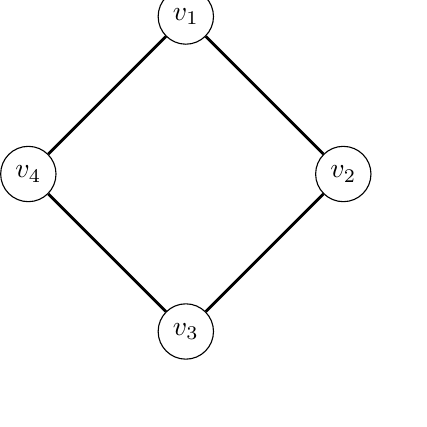
\begin{tikzpicture}[
        % ノードのスタイル設定
        mynode/.style={
            draw,           % 枠線を描画
            circle,         % 円形
            % fill=blue!20,   % 塗りつぶし色
            inner sep=2pt,  % 内側の余白
            minimum size=20pt % 最小サイズ
        },
        % 辺のスタイル設定
        myedge/.style={
            draw,           % 辺を描画
            line width=1pt  % 線の太さ
        }
    ]

    % ノードの定義と配置
    % polar座標を使って円形に配置します
    \node[mynode] (v1) at (90:2cm) {$v_1$};
    \node[mynode] (v2) at (0:2cm)  {$v_2$};
    \node[mynode] (v3) at (-90:2cm) {$v_3$};
    \node[mynode] (v4) at (180:2cm) {$v_4$};

    % 辺の定義
    \draw[myedge] (v1) -- (v2);
    \draw[myedge] (v2) -- (v3);
    \draw[myedge] (v3) -- (v4);
    \draw[myedge] (v4) -- (v1);

    \end{tikzpicture}
    \caption{$C_4$ グラフ}
    \label{fig:c4_graph}
\end{figure}

さて、区間グラフの定義から\(v_1\)と\(v_3\)、\(v_2\)と\(v_4\)は区間が重ならないようになっている。
そこで、\(v_1\)に対応する区間を\([s_{v_1}, e_{v_1}]\)、\(v_3\)に対応する区間を\([s_{v_3}, e_{v_3}]\)とする。
この時、区間は重ならないので\(e_{v_1} < s_{v_3}\)となる。
また、\(v_2\)と\(v_4\)はそれぞれ\(v_1\)と\(v_3\)の両方につながっているので区間が重なっている。
\(v_2\)に対応する区間を\([s_{v_2}, e_{v_2}]\)、\(v_4\)に対応する区間を\([s_{v_4}, e_{v_4}]\)とすれば上記の事実は\(s_{v_2}, s_{v_4} \in [s_{v_1}, e_{v_1}]\)かつ\(e_{v_2}, e_{v_4} \in [s_{v_3}, e_{v_3}]\)を満たすことに等しい。
すると\(v_2\)と\(v_4\)に対応する区間は重なることになるが、これは\(v_2\)と\(v_4\)の間に辺が引かれていないことに矛盾する。\\
\hspace{1em}故に\(C_4\)は区間グラフではない。
\end{proof}

\section{問3}
\hspace{1em}問4では\(C_4\)の彩色多項式を求める。
彩色多項式は以下の式によって再帰的に求まる。

\begin{equation}
  P_{C_4}(k) = P_{C_4 - e}(k) - P_{C_4 \backslash e}(k)
\end{equation}

目的の彩色多項式を求めるために、\(C_4\)から1つの辺を除去したグラフ\(C_4 - e\)と縮退したグラフ\(C_4 \backslash e\)の図を載せる。
\begin{figure}
    \centering
    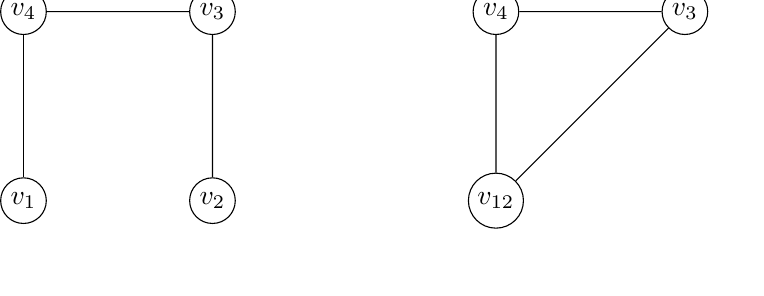
\begin{tikzpicture}[scale=1.2, every node/.style={circle, draw, fill=white, inner sep=2pt}]
      %--- 左: 辺{v1,v2}を除去 ---
      \node (v1) at (0,0)   {$v_1$};
      \node (v2) at (2,0)   {$v_2$};
      \node (v3) at (2,2)   {$v_3$};
      \node (v4) at (0,2)   {$v_4$};
      % \draw (v1) -- (v2); % この辺を除去
      \draw (v2) -- (v3);
      \draw (v3) -- (v4);
      \draw (v4) -- (v1);
      % \node at (1,-0.8) {除去};

      %--- 右: 辺{v1,v2}を縮退 ---
      % 横に4単位ずらす
      \node (v12) at (5,0)   {$v_{12}$};
      \node (w3)  at (7,2)   {$v_3$};
      \node (w4)  at (5,2)   {$v_4$};
      \draw (v12) -- (w3);
      \draw (w3) -- (w4);
      \draw (w4) -- (v12);
      % \node at (6,-0.8) {縮退};
    \end{tikzpicture}
    \caption{C$_4$の$\{v_1, v_2\}$を除去(左)・縮退(右)したグラフ}
\end{figure}

それぞれの彩色多項式を求めると
\begin{align}
  P_{C_4 - {v_1, v_2}}(k) &= k(k - 1)^3 \\
  P_{C_4 \backslash {v_1, v_2}}(k) &= k(k - 1)(k - 2)
\end{align}

となる。
従って\(C_4\)の彩色多項式は\(P_{C_4} = k(k - 1)(k^2 - 3k + 3)\)となる。

%%%%%%%%%%%%%%%%%%%%%%%%%%%%%%%%%%%%%%%%%%%%%%%%%%%%%%%%%%%%%%%%%%%%%%
\appendix
\setcounter{figure}{0}
\setcounter{table}{0}
\numberwithin{equation}{section}
\renewcommand{\thetable}{\Alph{section}\arabic{table}}
\renewcommand{\thefigure}{\Alph{section}\arabic{figure}}
%\def\thesection{付録\Alph{section}}
\makeatletter 
\newcommand{\section@cntformat}{付録 \thesection:\ }
\makeatother
%%%%%%%%%%%%%%%%%%%%%%%%%%%%%%%%%%%%%%%%%%%%%%%%%%%%%%%%%%%%%%%%%%%%%%

    
\end{document}
